\begin{figure}[H]
	\centering
	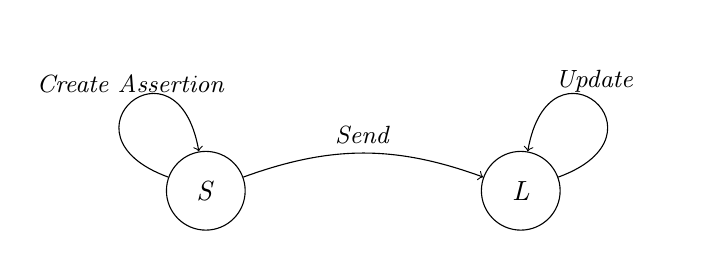
\begin{tikzpicture}[baseline=(S.base)]
		\tikzset{every loop/.style={min distance=10mm,looseness=10}}
		\node (S) at (0, 0) [shape=circle,draw,minimum size=1cm] {\textit{S}};
		\node (L) at (4, 0) [shape=circle,draw, minimum size=1cm] {\textit{L}};
		\path[->] (S) edge[bend left = 20] node[above]{\small \textit{Send}} (L)
		edge[loop above,in=100,out=160, min distance=8mm,looseness=8] node{\small \textit{Create Assertion}} (S)
		(L) edge[loop above,in=80,out=20, min distance=8mm,looseness=8] node{\small \textit{Update}} (L);
	\end{tikzpicture}
	\caption{Simple model of the interaction between two agents. \textit{S} is the speaker and \textit{L} is the listener. \textit{S} creates an argument that it then sends to \textit{L}. \textit{L} will then update its own beliefs according to the argument it receives from \textit{S}.}
	\label{fig:simple_interaction}
\end{figure}

Communication between two agents can be modelled as a simple sender-receiver model~\cite{Crawford1998ATalk}. A general form of this interaction has a sender/speaker, shown as \textit{S} in \cref{fig:simple_interaction}, communicating with a receiver/listener shown as \textit{L}. In  this model there are two parts that could be varied: Here we assume that the speaker has access to information about the listener, such as its beliefs and its update rule. This model can be used to explore the dynamics given minor variations in the assertion and the update rule. 

To initialise this model, each agent is assigned a probability distribution over each of the $n$ states of the world that can be enumerated due to the CWA. This is achieved by drawing $n-1$ values from a uniform distribution $ \mathbf{X}^{n-1} \sim \mathcal{U}(0,1)$, then sorting \textbf{X} in ascending order. The probability distribution $\mathbf{P}^n$ is then given by the size of the interval between these each consecutive pairs of points. This is akin to breaking a stick of length 1 in $n-1$ random places to give $n$ pieces. A population of $N$ agents is initialised in this way. At each time step, two agents are drawn from the population, one acting as speaker, one as listener. 

Once selected, there are a variety of ways for the speaker and listener to behave. These are given in the following models and comparing entropy, convergence, consensus as defined below.

\textbf{Definition 1: Entropy}. \textit{For each iteration $i$, the Shannon entropy measure $H$ can be averaged over each agent $j$ over each state of the world $k$ such that}

\begin{equation}\label{eq:shannon_entropy}
    H_i = - \frac{1}{N} \sum_j^N \sum_k^n p_{i, j, k} \cdot log(p_{i,j, k}).
\end{equation}

\textit{where $p_{i,j,k}$ is an agent $j$'s probability in state $k$ at the $i^\textnormal{th}$ iteration.}~\cite{Shannon1948ACommunication}


\textbf{Definition 2: Convergence. } \textit{Convergence $c_S$ is given by the iteration at which the change in entropy of the system over $t$ iterations is below a threshold $\epsilon$. This is given by}

\begin{equation}
    \Delta H = |H_i - H_t| \leq \epsilon
\end{equation}


\textbf{Definition 3: Consensus. } \textit{Consensus indicates the extent to which agents are in agreement at the time of convergence. It is given by the average pairwise J-divergence at convergence. This can be computed as}

\begin{equation}
    J = -\frac{1}{N}\sum_j^N \frac{1}{N} \sum_m^N \frac{1}{2} (D(p_{j}||M) + D(p_{m}||M)) 
\end{equation}
\textit{where $M = \frac{1}{2} (p_{j} + p_{m})$ and $D(\cdot || \cdot)$ is the KL-divergence. It is not sufficient to simply apply the KL-divergence due to its lack of symmetry invalidating it as a distance metric, but the J-divergence addresses this problem\cite{JohnsonSymmetrizingDistance}.} 

\subsection{The Open Model}
The first way we consider for a speaker to construct its assertion is for the agent so simply broadcast $\mathbf{P}^n$ to the listener, providing a precise description of the speakers beliefs about the state of the world. 

The listener agent then updates its beliefs at that timestep $\mathbf{P}^t_L$, such that

\begin{equation} \label{eq:simple_update_rule}
    \mathbf{P}^{i+1}_L = \alpha \cdot \mathbf{P}^{i}_L + (1 - \alpha) \cdot \mathbf{A}_S,
\end{equation}

where $\alpha \in [0, 1] $ denotes the listeners apathy or level of interest in new information, $i$ is the current timestep and $\mathbf{A}_S$ is the speaker's assertion. In this case, $\mathbf{A}_S$ is equivalent to the speaker's probability distribution. This gives

\begin{equation}
        \mathbf{P}^{i+1}_L = \alpha \cdot \mathbf{P}^{i}_L + (1 - \alpha) \cdot \mathbf{P}^{i}_S. \label{eq:fp_open}
\end{equation} 

